% Бүлэг 2

\chapter{Хичээлийн хуудас веб системийн шинжилгээний хэсэг} % Бүлгийн нэр
\label{Chapter2} % Энэ бүлэг рүү ишлэл хийх бол \ref{Chapter1} командыг ашигла 
\section{Системийг ашиглах хэрэглэгчид}

\begin{itemize}
\item Сургалтын албаны ажилтан
\item Багш
\item Оюутан
\item Эцэг эх

\end{itemize}
\section{Функциональ шаардлага}
Оюутан:
\begin{enumerate}
	\item Хичээлийн мэдээлэл харах
	\item Хөтөлбөрийн мэдээлэл харах
	\item Хайлт хийх
\end{enumerate}
Багш:
\begin{enumerate}
	\item Групп үүсгэх
	\item Пост оруулах 
\end{enumerate}
Сургалтын албаны ажилтан:
\begin{enumerate}
	\item Хичээл бүртгэх
	\item Ерөнхий хичээлийн групп үүсгэх
\end{enumerate}
Админ:
\begin{enumerate}
	\item Тайлан гаргах
\end{enumerate}
\section{Функциональ бус шаардлага}
\begin{enumerate}
	\item Интерфейс энгийн бөгөөд хэрэглэхэд ойлгомжтой байх
	\item Өгөгдлийн сан ачааллах хугацаа нь хурдан шуурхай байх
	\item Вебд үйл ажиллагаа явуулах серверийн хүчин чадал өндөр байх
	\item Бүх төрлийн төхөөрөмжөөс үзэхэд тохиромжтой хэлбэрээр харагддаг байх буюу загвар нь responsive байх
\end{enumerate}
\newpage
\section{Юзкейс диаграм}
\begin{figure}[htbp]
	\centering
	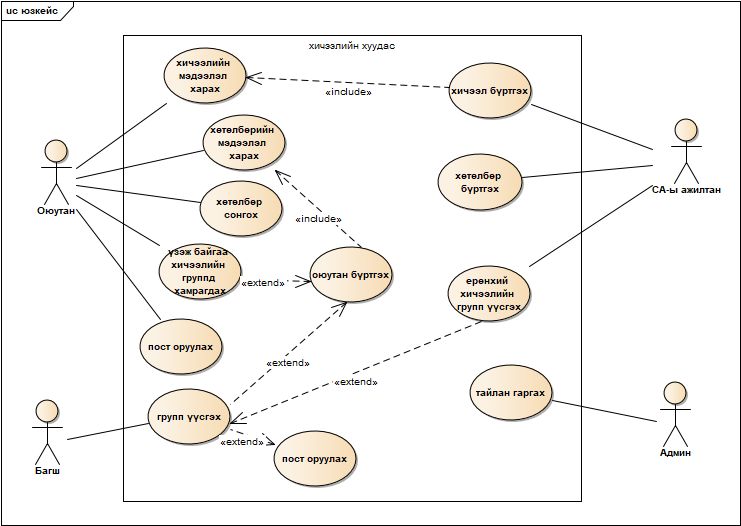
\includegraphics[angle=90,scale=0.65]{Diagrams/usecase.png}
	\caption[Юзкейс диаграм]{Юзкейс диаграм}
	\label{fit:UseCase}
\end{figure}
\newpage
\section{Юзкейс диаграмын тодорхойлолт}

\begin{center}
	\begin{table}[!htbp]
		\label{Хичээл бүртгэх}
		\begin{tabular}{|p{2cm}|p{13cm}|}
		\hline
			Нэр: & Хичээл бүртгэх \\
		\hline
			ID: & 1 \\
		\hline
			Товч тайлбар: & Хэрэглэгч бүртгэлээрээ хичээлийн  хуудсанд нэвтрэх. \\
		\hline
			Триггер: & - \\
		\hline
			Үндсэн оролцогч: & Хэрэглэгч-Сургалтын албаны ажилтан \\
		\hline
			Хоёрдогч оролцогч: & Байхгүй  \\
		\hline
			Өмнөх нөхцөл: &  Хэрэглэгч хичээлийн веб хуудсыг ачаалласан байх.\\
		\hline
			Ажлын урсгал: & \begin{enumerate}
						 	\item Хэрэглэгч “Хичээл бүртгэл”-ийг сонгосноор энэ юзкейс эхэлнэ. 
						 	\item Систем хэрэглэгчид бүртгэлийн хэсгийг харуулна. 
						 	\begin{enumerate}
						 		\item Хичээлийн нэр
						 		\item Хичээлийн код
						 		\item Хичээлийн кредит
						 		\item Хичээлийн дэлгэрэнгүй гэх мэт
						 	\end{enumerate}
						 	\item Хэрэглэгч бүртгэлийн хэсгийг бөглөөд хичээл нэмэхийг сонгоно. 
						 	\item Систем бүртгэлийн мэдээллийг зөв оруулсан эсэхийг шалгана.
						 	\item IF (бүргэл буруу бол)
							 	\begin{enumerate}
							 		\item[5.1]	Хэрэглэгчид буруу оруулсан байгааг анхааруулна, ахин зөв оруулахыг шаардана.
							 		\item[5.2] 5.2	Үндсэн урсгалын 2-р алхам руу шилжинэ. 
							 	\end{enumerate}
						 	\item ELSE
							 	\begin{enumerate}
							 		\item[6.1] Хэрэглэгч шинэ хичээл нэмнэ.
							 	\end{enumerate}
						  \end{enumerate}
\\					  \hline
				Дараах нөхцөл: &
				 \begin{enumerate}
									\item Хэрэглэгч системд нэвтэрсэн байна. 
									\item Хэрэглэгчийн мэдээлэл баазад хадгалагдсан байна. 
				\end{enumerate}	   
\\				   \hline
				Альтернатив урсгал: &  \begin{enumerate}
									\item Хэрэглэгч бүртгэлийг цуцалсан.
									\item Веб сервер дээр алдаа гарсан. 
										\end{enumerate}
				\\	\hline
		\end{tabular}
	\caption{Хичээл бүртгэх}
	\end{table}
\end{center}
\begin{center}
	\begin{table}[!htbp]
		\label{Групп үүсгэх}
		\begin{tabular}{|p{2cm}|p{13cm}|}
			\hline
			Нэр: & Групп үүсгэх \\
			\hline
			ID: & 1 \\
			\hline
			Товч тайлбар: & Хэрэглэгч бүртгэлээрээ хичээлийн  хуудсанд нэвтрэх. \\
			\hline
			Триггер: & - \\
			\hline
			Үндсэн оролцогч: & Хэрэглэгч-Сургалтын албаны ажилтан \\
			\hline
			Хоёрдогч оролцогч: & Байхгүй  \\
			\hline
			Өмнөх нөхцөл: &  Хэрэглэгч хичээлийн веб хуудсыг ачаалласан байх.\\
			\hline
			Ажлын урсгал: & \begin{enumerate}
				\item Хэрэглэгч “Хичээл групп”-ийг сонгосноор энэ юзкейс эхэлнэ. 
				\item Систем хэрэглэгчид бүртгэлийн хэсгийг харуулна. 
				\begin{enumerate}
					\item Группын нэр

				\end{enumerate}
				\item Хэрэглэгч бүртгэлийн хэсгийг бөглөөд групп нэмэхийг сонгоно. 
				\item Систем бүртгэлийн мэдээллийг зөв оруулсан эсэхийг шалгана.
				\item IF (бүргэл буруу бол)
				\begin{enumerate}
					\item[5.1]	Хэрэглэгчид буруу оруулсан байгааг анхааруулна, ахин зөв оруулахыг шаардана.
					\item[5.2] 5.2	Үндсэн урсгалын 2-р алхам руу шилжинэ. 
				\end{enumerate}
				\item ELSE
				\begin{enumerate}
					\item[6.1] Хэрэглэгч шинэ групп нэмнэ.
				\end{enumerate}
			\end{enumerate}
			\\					  \hline
			Дараах нөхцөл: &
			\begin{enumerate}
				\item Хэрэглэгч системд нэвтэрсэн байна. 
				\item Хэрэглэгчийн мэдээлэл баазад хадгалагдсан байна. 
			\end{enumerate}	   
			\\				   \hline
			Альтернатив урсгал: &  \begin{enumerate}
				\item Хэрэглэгч бүртгэлийг цуцалсан.
				\item Веб сервер дээр алдаа гарсан. 
			\end{enumerate}
			\\	\hline
		\end{tabular}
		\caption{Групп үүсгэх}
	\end{table}
\end{center}
%-------------------------------------------------------------------------------
\newpage
\section{Үйл ажиллагааны диаграм}
\begin{figure}
	\centering
	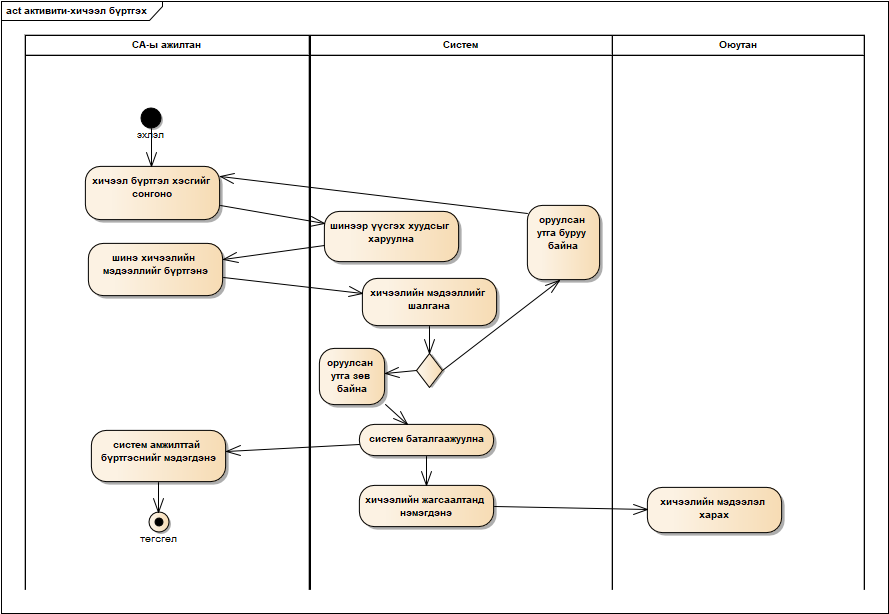
\includegraphics[angle=90, scale=0..]{Diagrams/activity-hicheelbvrtgel}
	\caption[Хичээл бүртгэх үйл ажиллагааны диаграм]{Хичээл бүртгэх үйл ажиллагааны диаграм}
	\label{text}
\end{figure}
\begin{figure}
	\centering
	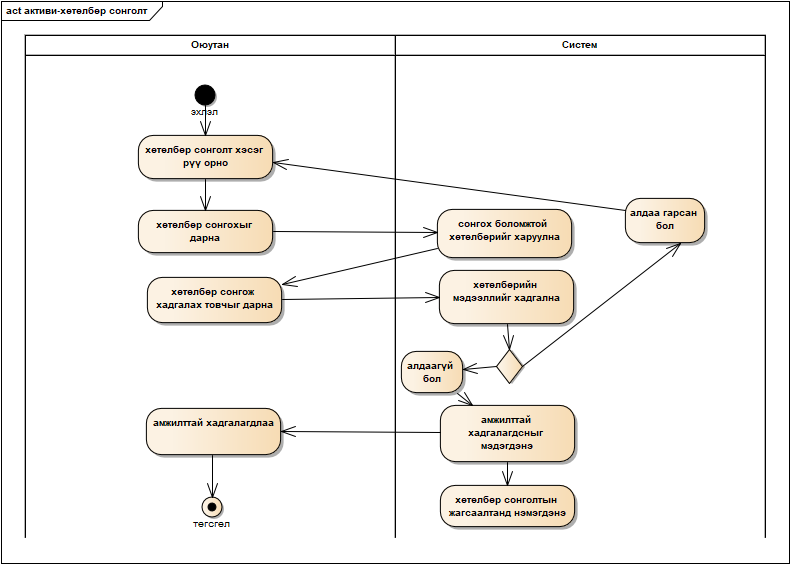
\includegraphics[angle=90, scale=0.65]{Diagrams/activity-hutulbursongolt}
	\caption[Хөтөлбөр сонголтын үйл ажиллагааны диаграм]{Хөтөлбөр сонголтын үйл ажиллагааны диаграм}
	\label{text}
\end{figure}

%--------------------------------------------------------------
\newpage
\section{Дарааллын диаграм}
\begin{figure}
	\centering
	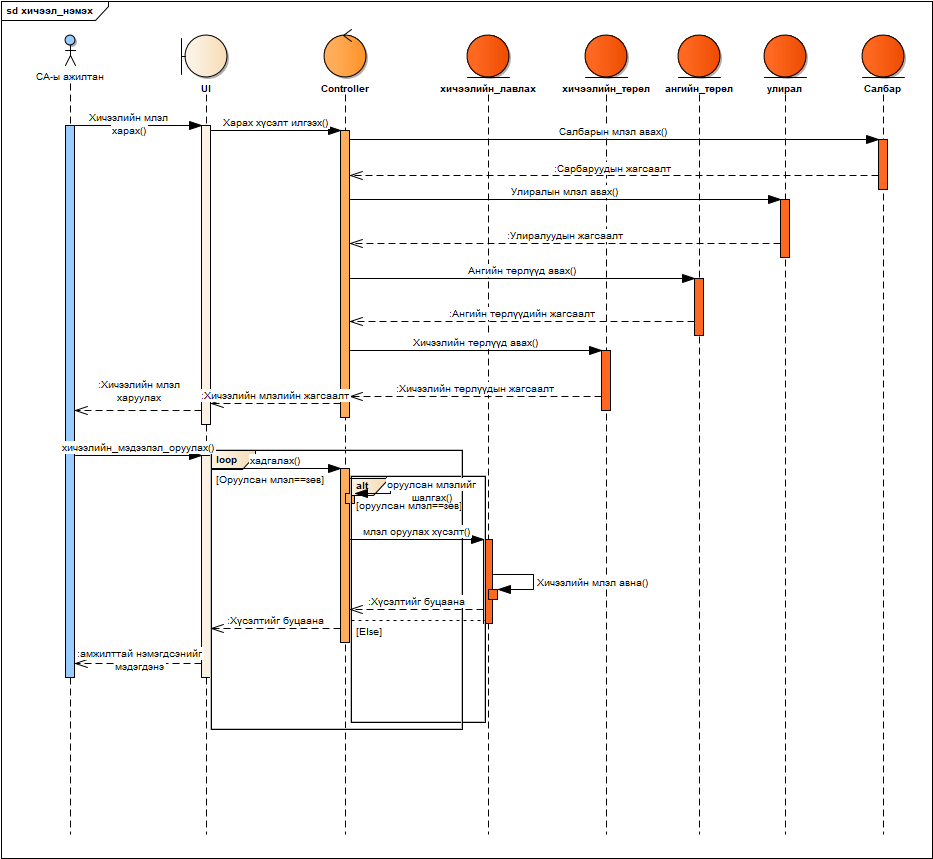
\includegraphics[angle=90,scale=0.6]{Diagrams/sequence_SA_ajiltan_hicheel_bvrtgeh}
	\caption[Хичээл бүртгэх дарааллын диаграм]{Хичээл бүртгэх дарааллын диаграм}
	\label{text}
\end{figure}
\begin{figure}
	\centering
	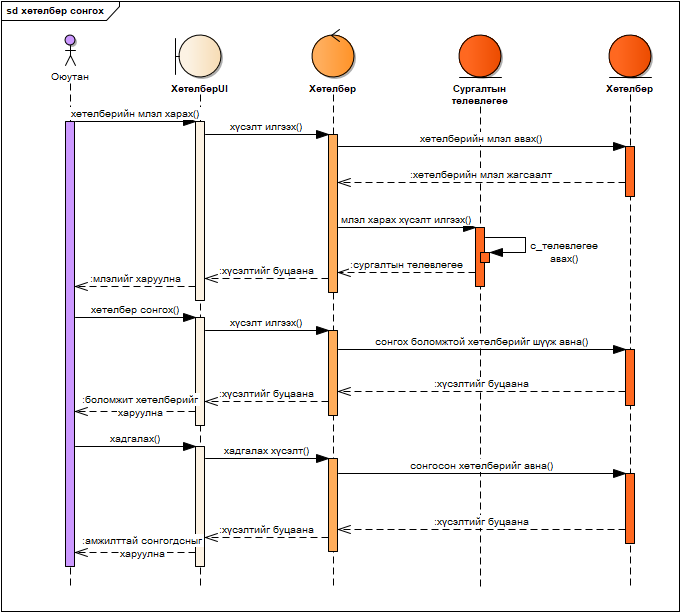
\includegraphics[angle=90,scale=0.65]{Diagrams/sequence_oyutan_hutulbur_songoh}
	\caption[Хөтөлбөр сонголтын дарааллын диаграм]{Хөтөлбөр сонголтын дарааллын диаграм}
	\label{text}
\end{figure}
\begin{figure}
	\centering
	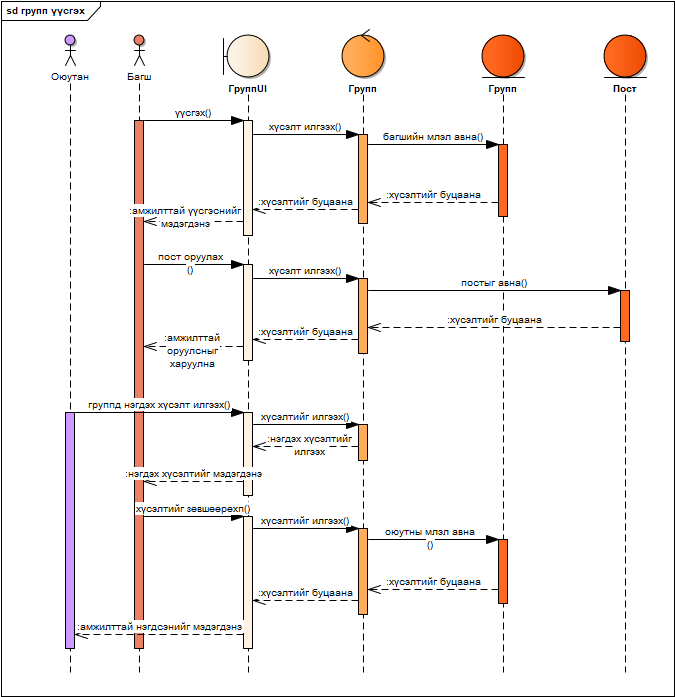
\includegraphics[angle=90, scale=0.65]{Diagrams/sequence_group_vvsgeh}
	\caption[Групп үүсгэх дарааллын диаграм]{Групп үүсгэх дарааллын диаграм}
	\label{text}
\end{figure}
\newpage
\section{Бүлгийн дүгнэлт}
Хэрэглэгчийн шаардлагаа тодорхойлж тодорхойлсон шаардлага бүрээ нягтлан хянаж функционал болон фунционал бусаар нь ялгасан. Функционал шаардлага дээрээ үндэслэн юзкейс диаграмаа гаргасан ба бүх  юзкейс бүрт тодорхойлолт гаргасан. Мөн тодорхойлолт бичсэн юзкейс диаграм бүртээ үйл ажиллагааны диаграм зурсан үйл ажиллагааг нь илүү нарийн ойлгомжтой болгож өгч байна.

